\documentclass[11pt,a4paper]{article}

\usepackage[utf8]{inputenc}
\usepackage[T1]{fontenc}
\usepackage[margin=1in]{geometry}
\usepackage{amsmath,amssymb,amsthm}
\usepackage{booktabs}
\usepackage{enumitem}
\usepackage{longtable,array,url,placeins}
\usepackage[hidelinks]{hyperref}
\usepackage[protrusion=true,expansion=false]{microtype}

\theoremstyle{plain}
\newtheorem{theorem}{Theorem}
\newtheorem{proposition}[theorem]{Proposition}
\theoremstyle{definition}
\newtheorem{definition}[theorem]{Definition}

\newcommand{\R}{\mathbb{R}}
\newcommand{\E}{\mathbb{E}}
\newcommand{\Var}{\operatorname{Var}}
\newcommand{\simplex}{\Delta^{m-1}}
\newcommand{\pipre}{\pi^{\mathrm{pre}}}
\newcommand{\pieq}{\pi^{\mathrm{eq}}}
\newcommand{\pir}{\pi^{r}}
\newcommand{\pihat}{\widehat{\pi}}
\newcommand{\epsincons}{\varepsilon_{\mathrm{incons}}}
\newcommand{\epssurr}{\varepsilon_{\mathrm{surr}}}
\newcommand{\epslearn}{\varepsilon_{\mathrm{learn}}}

\usepackage{graphicx}

\newcolumntype{L}[1]{>{\raggedright\arraybackslash}p{#1}}
\setlength{\emergencystretch}{2em}
\renewcommand{\topfraction}{0.9}
\renewcommand{\bottomfraction}{0.85}
\renewcommand{\textfraction}{0.1}
\renewcommand{\floatpagefraction}{0.7}
\title{\vspace{-1.5em}What Additive Risk-Adjusted Rewards Actually Optimise\\
in Reinforcement Learning for Asset Allocation}
\author{Matin Tavakoli}
\date{Research Proposal}
\begin{document}
\maketitle
\vspace{-1.5em}


\begin{abstract}

\noindent Financial reinforcement learning optimises the reward supplied to it, which need not induce the investor's intended terminal mean-variance policy. This project specifies the target policy first, solves the control problem induced by the reward, and separates reward-design mismatch from learning error. For independent returns and unconstrained risky dollar holdings, we establish the exact local mismatch coefficient of the scalar quadratic-increment reward for every fixed horizon, and construct a terminal-unit reward that recovers the mean-variance equilibrium. Exact benchmarks, adaptations of published reward formulas, and separate learning experiments quantify the scope and limits of the result. Policy alignment improves in the analytic setting, but the evidence does not establish universal improvement in Sharpe, initial mean-variance value, or learned performance. Existing mean-variance policy iteration already recovers the zero-interest scalar calibration; publication priority of the quantitative results remains open. This proposal presents the established results and identifies the remaining research.

\end{abstract}

\section{Problem, method and established contribution}

\subsection{The problem}
A financial RL agent optimises the reward supplied to it. A good Sharpe ratio or a well-trained policy does not establish that this reward represents the investor's intended terminal financial objective. The first decision is therefore which policy is intended: the initial-date mean--variance optimum, or the time-consistent equilibrium followed by successive decision makers.

\subsection{The method}
Specify the financial objective and target policy; solve the reward-induced control problem; measure policy mismatch independently of learning; calibrate or redesign the reward; then evaluate the learned policy against both exact references.

\subsection{The strongest established result}
For an unconstrained independent-return market, one scalar penalty on squared wealth increments cannot generally recover the terminal mean--variance equilibrium at nonzero interest. We derive its exact local mismatch coefficient for every fixed horizon, and give a terminal-unit excess-gain reward that recovers the equilibrium exactly. These are scoped mathematical results, not a claim of universal financial or learning superiority.

\begin{figure}[htbp]
\centering
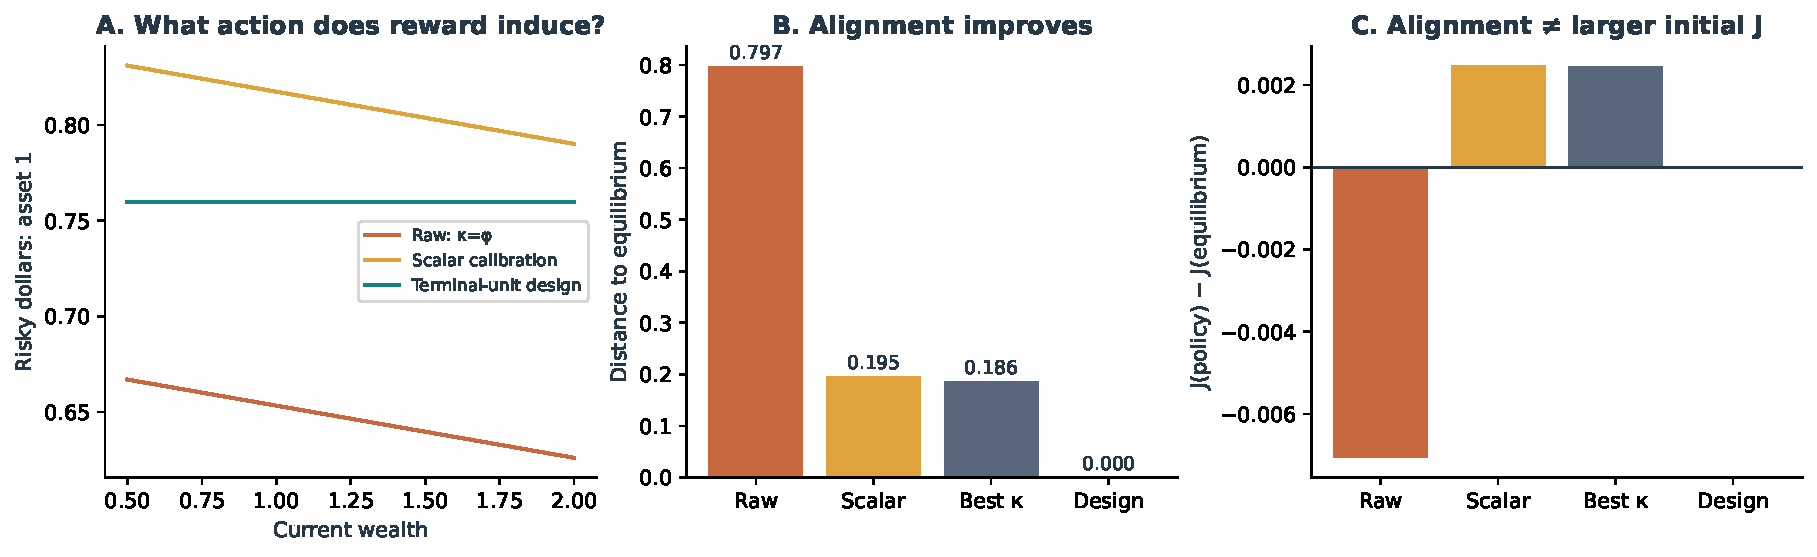
\includegraphics[width=\linewidth]{figures/01_policy_alignment.pdf}
\caption{NUMERICALLY VERIFIED. $T=4$, $\varphi=1$, $s=1.02$, three risky assets. Reward redesign eliminates exact policy mismatch. Scalar calibration attains a slightly larger initial J than equilibrium: better alignment and larger initial J are different goals.}
\label{fig:01_policy_alignment}
\end{figure}
Practical output: an auditable test of whether a portfolio reward targets the specified policy, a constructive correction when assumptions permit it, and a diagnosis of whether reward design or learning is the main remaining error.


\section{What the closest literature actually does}

The gap is not that financial RL ignores objectives or time inconsistency. Several important papers address them directly. The relevant question is how a specified reward's optimal policy differs from an independently specified terminal-wealth target.

\begingroup\small
\setlength{\LTpre}{8pt}\setlength{\LTpost}{8pt}
\renewcommand{\arraystretch}{1.18}
\begin{longtable}{@{}L{\dimexpr 0.300\linewidth-1.200\tabcolsep\relax}L{\dimexpr 0.350\linewidth-1.400\tabcolsep\relax}L{\dimexpr 0.350\linewidth-1.400\tabcolsep\relax}@{}}
\toprule
\textbf{Paper / exact locator} & \textbf{Objective and method} & \textbf{Role in this project}\\
\midrule\endfirsthead
\toprule
\textbf{Paper / exact locator} & \textbf{Objective and method} & \textbf{Role in this project}\\
\midrule\endhead
\bottomrule\endfoot
Kolm--Ritter (2019), manuscript Eqs. 8--10 & Approximate quadratic increment reward; fitted SARSA hedging. & Closest reward family; explicitly acknowledges covariance/approximation.\\[3pt]
Jiang et al. (2017), \S{}4.2 Eqs. 21--22 & Log-growth reward; direct gradient portfolio learning. & Alternative preference; not intrinsically a wrong growth reward.\\[3pt]
Yang et al. (2020), \S{}3.3 Eq. 4; Table 2 & Net value change; PPO/A2C/DDPG; Sharpe ensemble selection. & Return-reward adaptation; separates reward from evaluation criterion.\\[3pt]
Moody--Saffell (2001), \S{}II-D Eqs. 14--15 & Differential Sharpe; recurrent direct reinforcement. & Augmented-state DSR comparison, not fixed-penalty equivalence.\\[3pt]
Bisi et al. (2020), \S{}\S{}3--5; Zhang et al. (2021), Algorithm 1 & Per-step mean-volatility; TRVO / MVPI-TD3. & Direct prior reward-transformation theory; MVPI adaptation added.\\[3pt]
Wang--Zhou (2020), \S{}2 Eq. 11; Dai et al. (2023), working \S{}4 & Objective-specific MV RL; precommitment / log-MV equilibrium. & Positive precedents with analytic references; no first-MV-RL claim.\\[3pt]
\end{longtable}
\endgroup

Concrete positioning: Kolm--Ritter optimise an explicitly approximate quadratic increment reward for hedging. Jiang et al. choose log growth. Yang et al. train on value increments and select agents by Sharpe. Our benchmark holds the market and feasible set fixed, solves these adapted reward problems, and compares their induced policies with a prescribed mean--variance equilibrium. This tests preference alignment; it does not refute each paper's own stated objective. \cite{ref1,ref2,ref3}

The zero-interest calibration is not a sufficient novelty claim: the finite-horizon iid reduction of Zhang's MVPI has the same fixed point. Basak--Chabakauri also discuss recovering time-consistent objectives with the same policy, and Björk--Murgoci's abstract states an associated-control result. The candidate contribution is the explicit quantitative obstruction and its audited removal within a concrete reward family. Priority remains OPEN. \cite{ref6,ref10,ref12}

The source ledger records authors, exact titles, venue, identifiers, reward, algorithm, data, reported results, and version-specific locators for every comparison. Eleven primary versions were inspected; one additional source is explicitly abstract-only.


\section{Objective, benchmark and calibration procedure}

Established analytic scope: finite horizon T, initial wealth $x_0$, deterministic positive risk-free gross returns $s_t$, unconstrained risky dollar holdings $u_t$, and independent excess-return vectors $P_t$ with means $m_t$ and positive-definite covariances $\Sigma_t$. Gaussian sampling is used for training, but the exact affine moment results only require finite second moments. Long-only weights are treated separately.

\begin{equation}
\begin{aligned}
 X_{t+1}&=s_tX_t+P_t^{\top}u_t,& J(\pi)&=\E[X_T]-\varphi\Var(X_T),\quad\varphi>0,\\
 M_t&=\Sigma_t+m_tm_t^{\top},& d_t&=M_t^{-1}m_t,\quad\nu_t=m_t^{\top}d_t<1,\\
 H_t&=\prod_{j=t+1}^{T-1}s_j,&u_t^{\mathrm{eq}}&=\frac{\Sigma_t^{-1}m_t}{2\varphi H_t}.
 \end{aligned}
\end{equation}
Li--Ng supply the precommitted reference; equilibrium control follows consistent planning. Our redesign targets equilibrium. If initial-date performance is the intended objective, use the precommitted benchmark and an appropriate terminal objective instead. \cite{ref9,ref10,ref7}

\subsection{A reward-design rule with an explicit guarantee}
\begin{equation}
Y_t=H_tP_t^{\top}u_t,\qquad r_t^{\mathrm{design}}=Y_t-\varphi(1-\nu_t)Y_t^2.
\end{equation}
PROVED: conditional expected reward is strictly concave in $u_t$, wealth-independent, and maximised at $u_t^{\mathrm{eq}}$. Independence and unconstrained actions make these pointwise maximisers globally optimal for the additive reward. Scaling gains into terminal units removes the interest-driven obstruction of the original wealth-increment reward. Time-varying moments require date-specific calibration.

\begin{figure}[htbp]
\centering
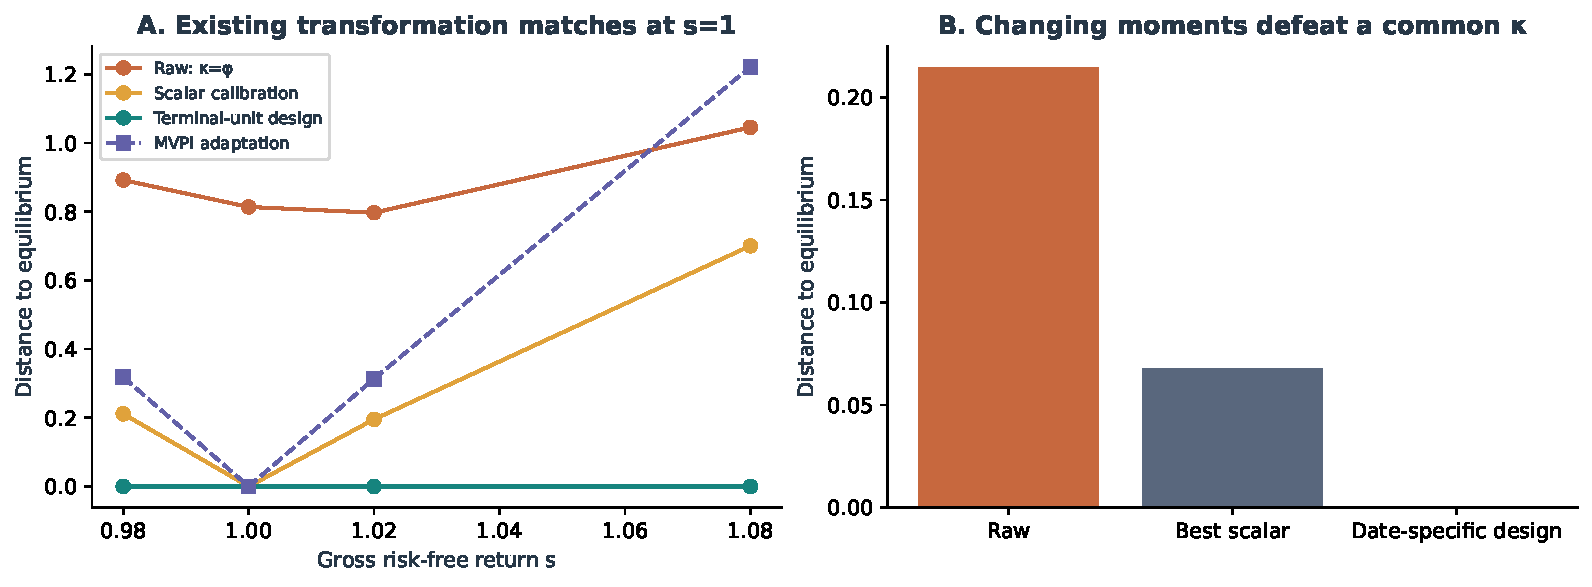
\includegraphics[width=\linewidth]{figures/10_existing_transformations.pdf}
\caption{NUMERICALLY VERIFIED. Existing MVPI adaptation agrees at zero interest but targets per-step mean-volatility away from it. With changing moments at zero interest, a common scalar penalty leaves distance 0.067715; the date-specific design gives zero.}
\label{fig:10_existing_transformations}
\end{figure}
Implementation procedure: estimate or specify moments; declare the target and constraints; solve the exact reward problem where possible; report distance and terminal J; optimise reward parameters using a fixed reference occupancy; then train with the resulting reward and report its optimisation error separately.


\section{Theoretical contribution and its boundaries}

\subsection{The irreducible raw-reward mismatch --- PROVED}
For iid returns set $d=M^{-1}m$, $\nu=m^{\top}d$ and $b=1/[2\varphi(1-\nu)]$. Assume $m\ne0$ and fixed $T\ge2$. For $r=\Delta X-\kappa(\Delta X)^2$, let D be the square root of summed expected squared action differences along the reward policy. Then, locally around $s=1$:

\begin{equation}
\begin{aligned}
 \min_{\kappa>0}D(\pi^{\kappa},\pieq)&=c_T|s-1|+O((s-1)^2),\\
 c_T&=\|d\|b\sqrt{\frac{T(T^2-1)}{3}+\frac{\nu(1-\nu)T(T-1)}{2}}.
 \end{aligned}
\end{equation}
At zero interest exact matching requires $\kappa=\varphi(1-\nu)$. At nonzero interest and $T\ge2$ the final reward-optimal policy has wealth slope $-d(s-1)$, while equilibrium has zero slope and reachable wealth has positive variance. No scalar $\kappa$ removes that difference. The statement concerns this reward family, not all additive rewards.

The proof closes the earlier remainder and minimisation gaps: write $h=1/(2\kappa)$; policy intercepts and controlled wealth are affine in h, so $D^2$ is exactly quadratic in h. Its coefficients are analytic in $s-1$ and its unique minimum remains interior near zero. This establishes the expansion after minimisation. At large fixed-parameter T, $c_T$ grows as $T^{3/2}$; this is not a joint uniform small-interest/large-horizon theorem.

\begin{figure}[htbp]
\centering
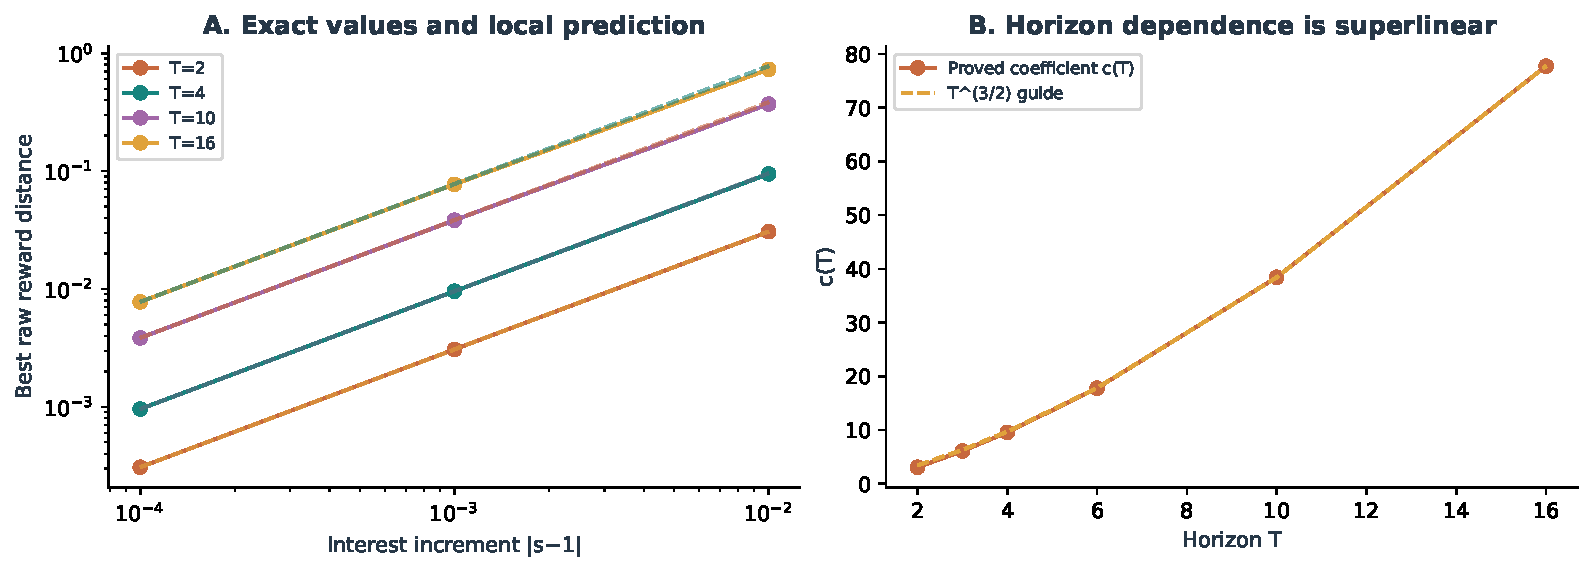
\includegraphics[width=\linewidth]{figures/02_horizon_theorem.pdf}
\caption{PROVED coefficient with NUMERICALLY VERIFIED finite-interest checks. Solid curves show exact calibration and dashed curves the local prediction. The earlier ``approximately linear in horizon'' claim is withdrawn.}
\label{fig:02_horizon_theorem}
\end{figure}
\subsection{Changing moments and a common penalty --- PROVED}
\begin{equation}
\begin{gathered}
 s_t=1:\qquad\min_{\kappa>0}D^2=\sum_{t=0}^{T-1}a_t(b_t-\bar b)^2,\\
 a_t=\|d_t\|^2,\qquad b_t=\frac{1}{2\varphi(1-\nu_t)},\qquad
 \bar b=\frac{\sum_t a_tb_t}{\sum_t a_t}.
 \end{gathered}
\end{equation}
The lower bound is positive exactly when $b_t$ varies across positive-weight dates. Time variation by itself is insufficient. Degenerate zero means, the positivity condition for one-period matching, and the local nature of the theorem are retained in the proof appendix.


\section{Fair comparison with published reward designs}

NUMERICALLY VERIFIED: a separate long-only benchmark has $T=3$, $x_0=1$, $s=1.02$, one risky excess return $-$.18 or .30 with equal probability, zero costs, and a common 21-point weight grid in [0,1]. Bellman recursion exhaustively solves each finite reward tree. DSR state includes A and B. A one-step-game recursion solves the equilibrium on the same grid. The 11-point grid is also run.

\begin{figure}[htbp]
\centering
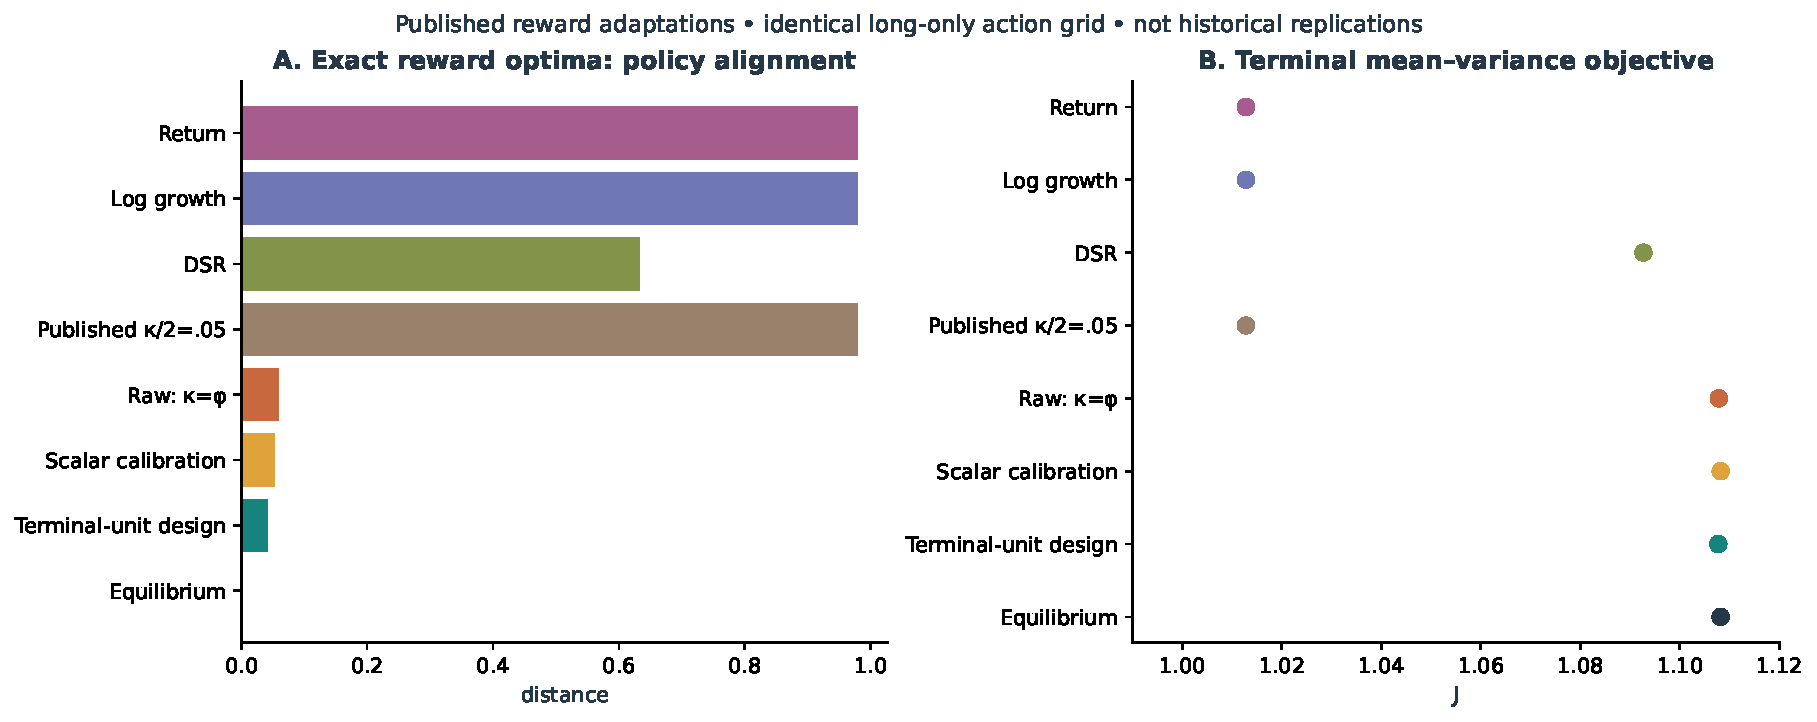
\includegraphics[width=\linewidth]{figures/04_published_rewards.pdf}
\caption{Adaptations of published formulas, not replications of their data, algorithms or reported performance. $\kappa/2=.05$ is a unit-sensitive coefficient copied from the Kolm--Ritter example and is shown only as a sensitivity diagnostic.}
\label{fig:04_published_rewards}
\end{figure}
\begingroup\small
\setlength{\LTpre}{8pt}\setlength{\LTpost}{8pt}
\renewcommand{\arraystretch}{1.18}
\begin{longtable}{@{}L{\dimexpr 0.430\linewidth-2.580\tabcolsep\relax}L{\dimexpr 0.190\linewidth-1.140\tabcolsep\relax}L{\dimexpr 0.190\linewidth-1.140\tabcolsep\relax}L{\dimexpr 0.190\linewidth-1.140\tabcolsep\relax}@{}}
\toprule
\textbf{Adapted reward} & \textbf{Distance} & \textbf{Terminal J} & \textbf{Excess Sharpe}\\
\midrule\endfirsthead
\toprule
\textbf{Adapted reward} & \textbf{Distance} & \textbf{Terminal J} & \textbf{Excess Sharpe}\\
\midrule\endhead
\bottomrule\endfoot
Value change & 0.97894 & 1.012819 & 0.39950\\[3pt]
Log growth & 0.97894 & 1.012819 & 0.39950\\[3pt]
DSR & 0.63257 & 1.092687 & 0.43313\\[3pt]
Published .05 diagnostic & 0.97894 & 1.012819 & 0.39950\\[3pt]
Raw $\kappa=\varphi$ & 0.05848 & 1.107849 & 0.43275\\[3pt]
Scalar calibration & 0.05313 & 1.108217 & 0.43368\\[3pt]
Terminal-unit design & 0.04137 & 1.107729 & 0.43138\\[3pt]
Grid equilibrium & 0.00000 & 1.108204 & 0.43369\\[3pt]
\end{longtable}
\endgroup

The design improves alignment over raw and scalar rewards in this configuration, but has slightly lower J than either. It does not exactly recover the constrained equilibrium: wealth-dependent feasible dollar holdings invalidate the unconstrained proof. Return and log-growth policies pursue different preferences, so their terminal-MV rankings are not evidence that they fail at their own tasks.

DSR uses $\eta=.1$, $A_0=.01$, $B_0=.01$ here. Sensitivity tests vary all three. Reward shapes are transferred; PPO/DDPG, RRL, trading costs, historical datasets and original train/test protocols are not reproduced. Algorithms cannot be ranked from this experiment.


\ifdim\dimexpr\pagegoal-\pagetotal\relax<150pt\newpage\fi

\section{Exact values, dependent returns and DSR}

\begingroup\small
\setlength{\LTpre}{8pt}\setlength{\LTpost}{8pt}
\renewcommand{\arraystretch}{1.18}
\begin{longtable}{@{}L{\dimexpr 0.430\linewidth-2.580\tabcolsep\relax}L{\dimexpr 0.190\linewidth-1.140\tabcolsep\relax}L{\dimexpr 0.190\linewidth-1.140\tabcolsep\relax}L{\dimexpr 0.190\linewidth-1.140\tabcolsep\relax}@{}}
\toprule
\textbf{Independent benchmark} & \textbf{Policy distance} & \textbf{Terminal J} & \textbf{Excess Sharpe}\\
\midrule\endfirsthead
\toprule
\textbf{Independent benchmark} & \textbf{Policy distance} & \textbf{Terminal J} & \textbf{Excess Sharpe}\\
\midrule\endhead
\bottomrule\endfoot
Precommitted reference & 3.312087 & 1.425799 & 1.171951\\[3pt]
Equilibrium & 0.000000 & 1.323644 & 0.982266\\[3pt]
Raw $\kappa=\varphi$ & 0.797127 & 1.316580 & 0.987285\\[3pt]
Scalar calibration & 0.195347 & 1.326115 & 0.987292\\[3pt]
Best scalar in raw family & 0.186435 & 1.326093 & 0.987292\\[3pt]
Terminal-unit design & 0.000000 & 1.323644 & 0.982266\\[3pt]
\end{longtable}
\endgroup

NUMERICALLY VERIFIED: $T=4$, $\varphi=1$, $s=1.02$. Distance falls from .797127 to .195347 after zero-interest scalar calibration and to numerical zero after redesign. Raw reward has higher excess Sharpe than equilibrium (.987285 vs .982266), but lower J (1.316580 vs 1.323644). Sharpe uses excess terminal gain over $x_0s^T$ and is not annualised.

\subsection{Dependence introduces an intertemporal hedge --- PROVED}
\begin{equation}
u^{\mathrm{eq}}(t,z)=\frac{m_z}{2\varphi H_t\Var(P\mid z)}
 -\frac{\operatorname{Cov}(P,a_{t+1}(z_{t+1})\mid z)}{H_t\Var(P\mid z)}.
\end{equation}
In the observed finite-regime model, $a_{t+1}$ is the expected terminal continuation gain. A calibration using only current conditional moments omits this covariance. Adding $-2\varphi H_tu\allowbreak\operatorname{Cov}(P,a_{t+1}\mid z)$ to the terminal-unit reward recovers equilibrium. This is an oracle construction using an already solved continuation, not a model-free learning result or a novel hedging principle. \cite{ref10}

\begin{figure}[htbp]
\centering
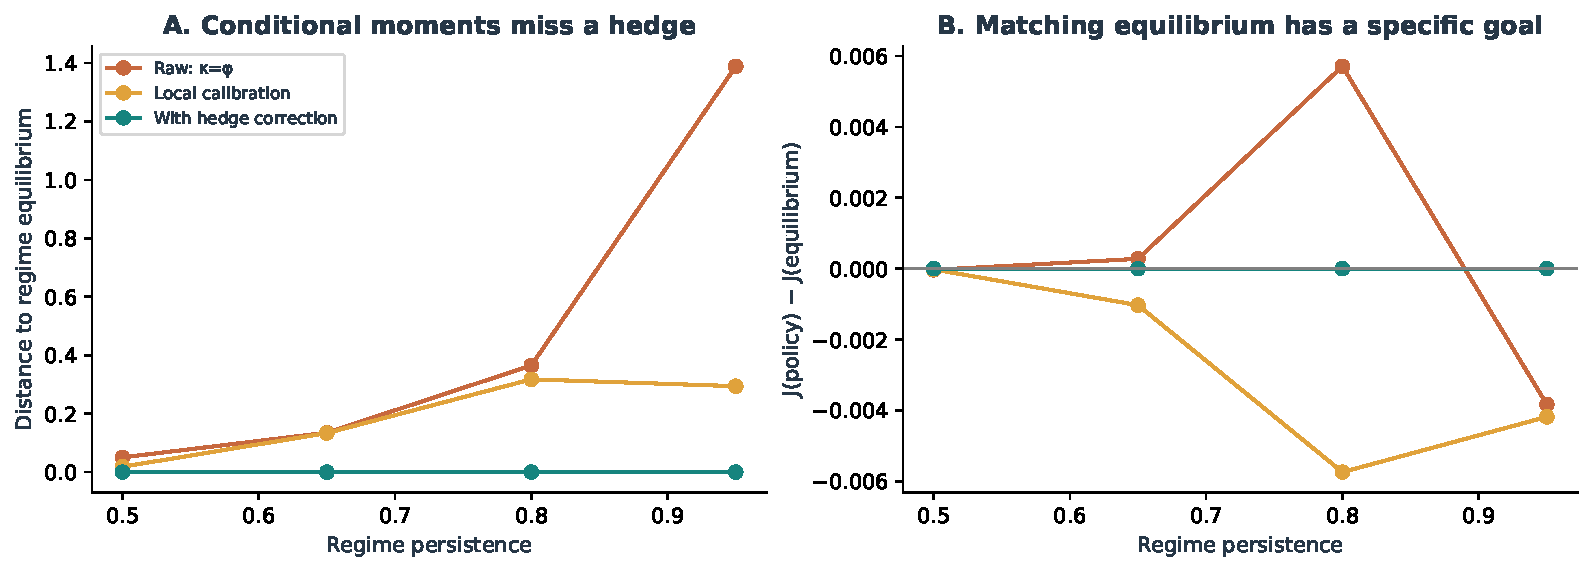
\includegraphics[width=\linewidth]{figures/05_dependent_returns.pdf}
\caption{NUMERICALLY VERIFIED exact joint return/regime recursion. At persistence .8, raw distance is .365102, local calibration .317644, hedge-corrected reward numerical zero. Raw J exceeds equilibrium J here; that is consistent with the target being equilibrium.}
\label{fig:05_dependent_returns}
\end{figure}
R6 --- PROVED: bounded finite-horizon DSR is well posed with state augmentation and $B_0-A_0^2>0$. Its local quadratic identity does not establish dynamic equivalence to a fixed variance penalty. Fixed-decay EWMA has positive limiting variance; the earlier consistency claim is false. Unrestricted or infinite-horizon DSR remains OPEN.


\section{Robustness and the limits of transfer}

\begin{figure}[htbp]
\centering
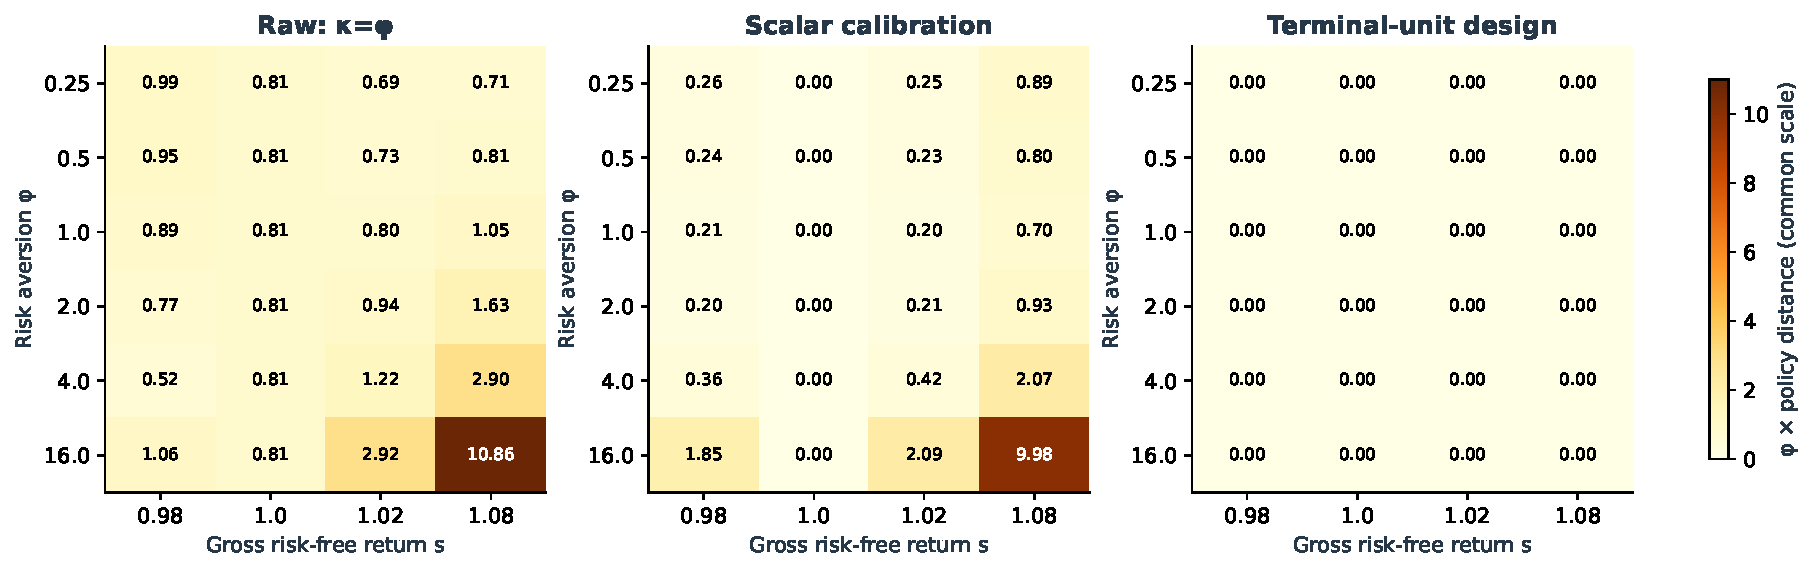
\includegraphics[width=\linewidth]{figures/03_risk_regimes.pdf}
\caption{NUMERICALLY VERIFIED. Common-scale $\varphi\times\text{distance}$ across risk aversion and interest. The full grid has 120 parameter configurations: five horizons, six risk aversions and four rates, each with six exact reference/reward policies. Maximum redesign discrepancy is $2.35\times10^{-14}$.}
\label{fig:03_risk_regimes}
\end{figure}
Additional exact checks vary mean, volatility and correlation over 27 markets. Redesign discrepancy remains below $5.50\times10^{-15}$. These verify the scoped identity, not robustness of estimated models to arbitrary market misspecification.

\begin{figure}[htbp]
\centering
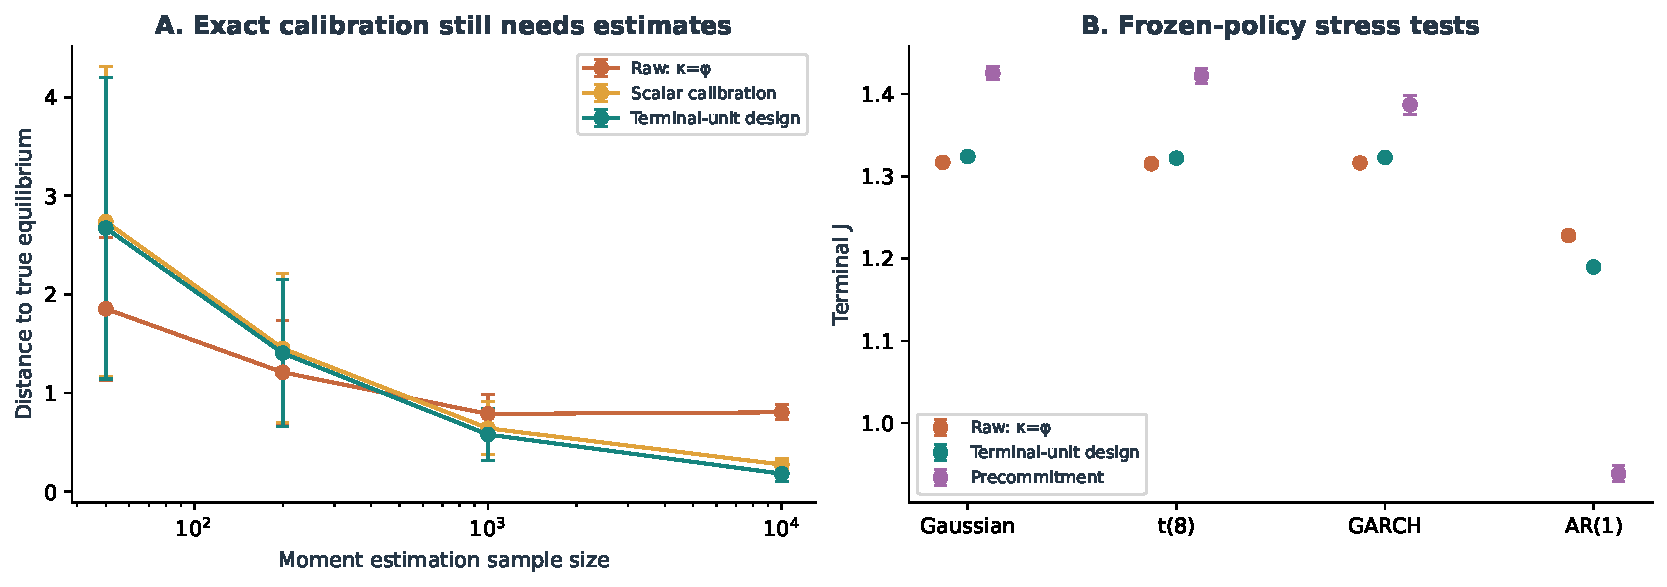
\includegraphics[width=\linewidth]{figures/08_estimation_robustness.pdf}
\caption{PRELIMINARY. Left: thirty independent moment-estimation samples at each size, mean $\pm$ sample SD. Right: frozen policies on ten batches of 50,000 paths, mean $\pm$ sample SD. GARCH and AR(1) are dependent stress tests; iid optimality is not asserted there.}
\label{fig:08_estimation_robustness}
\end{figure}
The design needs accurate moments. Estimation experiments evaluate policies built from estimated moments in the true market. Stress tests hold policies fixed: matched-moment iid t(8) preserves the moment-based result, but serial correlation can reverse performance. Under AR(1), design minus raw J is $-$.03813 (batch SE .00027); under Gaussian iid it is +.00713 (SE .00018). No universal robustness advantage is claimed.


\section{Separate learning error from reward-design error}

\begin{equation}
\begin{aligned}
 J(\pipre)-J(\pihat)
 &=\underbrace{J(\pipre)-J(\pieq)}_{\text{price of time consistency}}\\
 &\quad+\underbrace{J(\pieq)-J(\pir)}_{\text{signed reward-design difference}}\\
 &\quad+\underbrace{J(\pir)-J(\pihat)}_{\text{signed learning difference}}.
 \end{aligned}
\end{equation}
The identity telescopes. Only the first term is guaranteed nonnegative in this benchmark. The last two are signed differences in the financial objective. Report a separate nonnegative surrogate regret: expected reward at its exact optimum minus expected reward of the learned policy. Policy distance always uses the declared reference occupancy.

\begin{figure}[htbp]
\centering
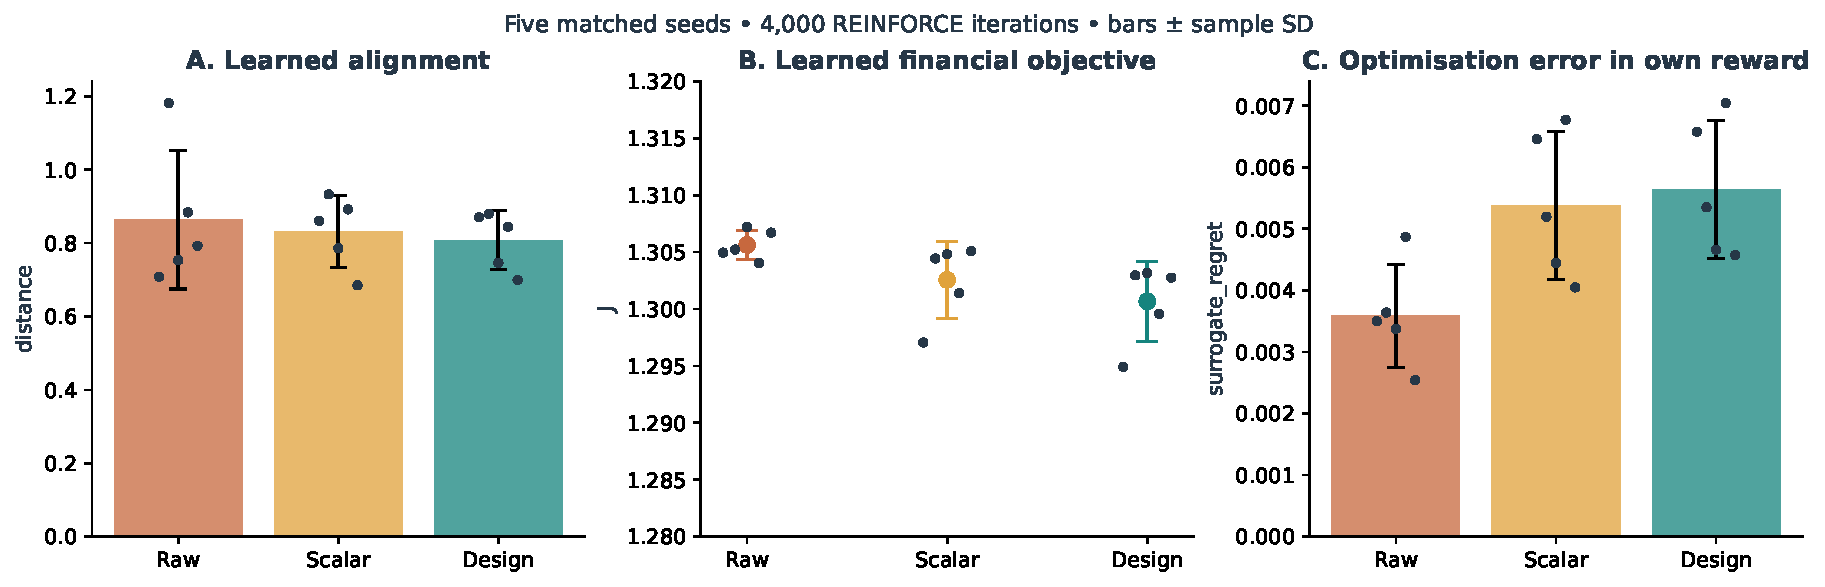
\includegraphics[width=\linewidth]{figures/06_learning_error.pdf}
\caption{PRELIMINARY. Five paired seeds per reward, 4,000 iterations and batches of 512, common affine policy family, Adam learning rate .02 and exploration schedule. This is the existing REINFORCE-style implementation with normalised advantages and scaled scores. No convergence theorem is asserted.}
\label{fig:06_learning_error}
\end{figure}
\begingroup\small
\setlength{\LTpre}{8pt}\setlength{\LTpost}{8pt}
\renewcommand{\arraystretch}{1.18}
\begin{longtable}{@{}L{\dimexpr 0.180\linewidth-1.080\tabcolsep\relax}L{\dimexpr 0.280\linewidth-1.680\tabcolsep\relax}L{\dimexpr 0.340\linewidth-2.040\tabcolsep\relax}L{\dimexpr 0.200\linewidth-1.200\tabcolsep\relax}@{}}
\toprule
\textbf{Learned reward} & \textbf{Mean distance $\pm$ SD} & \textbf{Mean J $\pm$ SD} & \textbf{Mean surrogate regret}\\
\midrule\endfirsthead
\toprule
\textbf{Learned reward} & \textbf{Mean distance $\pm$ SD} & \textbf{Mean J $\pm$ SD} & \textbf{Mean surrogate regret}\\
\midrule\endhead
\bottomrule\endfoot
raw & 0.8638 $\pm$ 0.1890 & 1.305628 $\pm$ 0.001303 & 0.003584\\[3pt]
scalar & 0.8312 $\pm$ 0.0978 & 1.302556 $\pm$ 0.003415 & 0.005381\\[3pt]
design & 0.8079 $\pm$ 0.0807 & 1.300671 $\pm$ 0.003543 & 0.005640\\[3pt]
\end{longtable}
\endgroup

The exact redesign is aligned, but the learned redesign retains substantial distance. Its mean J is lower than the learned raw reward at this budget. Thus the current learning experiment does not support improved financial performance or broad algorithmic superiority. Reward regret is reported in each reward's own units; comparisons of its scale across rewards require care.

The fair next algorithm study must tune each reward on a separate validation budget, keep environment interactions and policy capacity comparable, add seeds, and report uncertainty and failures. The current experiment is a diagnosis, not a finished PPO/DDPG benchmark.


\ifdim\dimexpr\pagegoal-\pagetotal\relax<150pt\newpage\fi

\section{What is established, and what remains proposed}

\begingroup\small
\setlength{\LTpre}{8pt}\setlength{\LTpost}{8pt}
\renewcommand{\arraystretch}{1.18}
\begin{longtable}{@{}L{\dimexpr 0.370\linewidth-1.480\tabcolsep\relax}L{\dimexpr 0.200\linewidth-0.800\tabcolsep\relax}L{\dimexpr 0.430\linewidth-1.720\tabcolsep\relax}@{}}
\toprule
\textbf{Result} & \textbf{Status} & \textbf{Boundary}\\
\midrule\endfirsthead
\toprule
\textbf{Result} & \textbf{Status} & \textbf{Boundary}\\
\midrule\endhead
\bottomrule\endfoot
R1 \textperiodcentered{} Raw reward recursion and zero-interest match & PROVED & Known control tools; zero-interest result also follows from MVPI.\\[3pt]
R2 \textperiodcentered{} Fixed-horizon mismatch coefficient & PROVED & Project derivation; literature priority not established.\\[3pt]
R3 \textperiodcentered{} Terminal-unit independent-return redesign & PROVED & Unconstrained dollar actions; known moments; equilibrium target.\\[3pt]
R4 \textperiodcentered{} Common-penalty lower bound under changing moments & PROVED & Zero interest; nonzero-mean dates; weighted dispersion formula.\\[3pt]
R5 \textperiodcentered{} Observed-regime hedge and oracle correction & PROVED & Scalar risky return, exogenous observed regimes; solved continuation required.\\[3pt]
R6 \textperiodcentered{} DSR algebra and finite-horizon well-posedness & PROVED & Bounded returns, positive initial EWMA variance; no infinite-horizon theorem.\\[3pt]
R7 \textperiodcentered{} Reward adaptations and parameter sweeps & NUMERICALLY VERIFIED & Exact recursions / exact finite action trees in specified markets.\\[3pt]
R8 \textperiodcentered{} Training and estimation evidence & PRELIMINARY & Five training seeds; thirty estimation seeds; no broad superiority claim.\\[3pt]
\end{longtable}
\endgroup

\subsection{What can a researcher do now?}
Audit an additive financial reward against a specified equilibrium, compute its exact induced policy and mismatch without learning noise, choose the best scalar penalty in the raw family, and determine whether a structural redesign is required. Under independent known moments, implement the displayed reward to recover equilibrium exactly. Under observable dependence, identify the missing continuation hedge rather than assume local calibration suffices.

\subsection{Remaining research, with acceptance criteria}
OPEN --- Publication priority: obtain the full discrete-control prior and compare the exact coefficient and redesign with earlier inverse-control and risk-sensitive RL results. Claim no ``first'' result before this is done. Existing MVPI equivalence must remain in the final positioning.

OPEN --- Constraints and costs: derive or numerically solve reward designs for wealth-dependent feasible sets, transaction costs and multiple dependent assets. Require a shared feasible benchmark and a quantified discretisation error before claiming exact recovery.

OPEN --- DSR: analyse unrestricted policies or an appropriately regularised infinite-horizon formulation. A bounded finite-grid calculation cannot establish a constant implied terminal risk aversion or a global DSR theorem.

PROPOSED --- Learning and practical validation: expand tuned policy-gradient, PPO and DDPG comparisons, implement estimated continuation hedges, and test with a preregistered historical protocol. Success means improved target alignment with controlled learning error; Sharpe and raw return remain secondary, separately reported outcomes.

The former general-horizon conjecture is resolved locally. The broad global Lambda inequality is withdrawn.


\clearpage

\section{Evidence that changes the interpretation}

\begin{figure}[htbp]
\centering
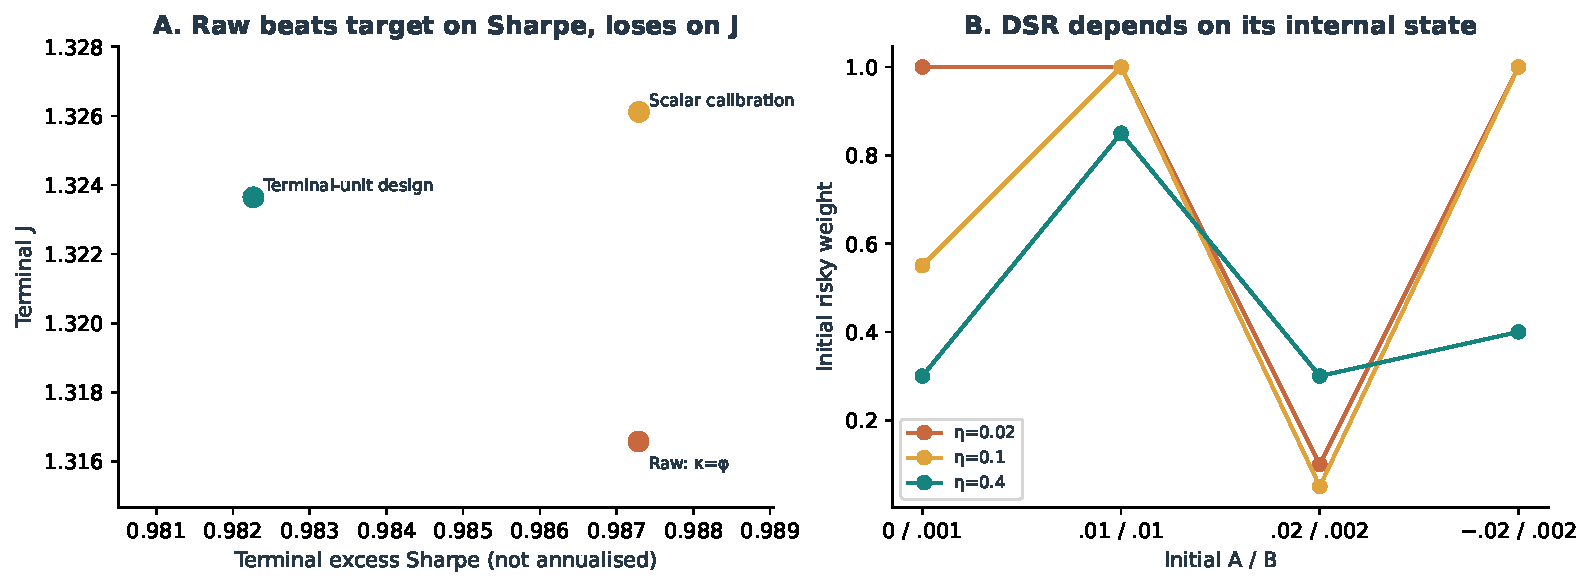
\includegraphics[width=\linewidth]{figures/07_sharpe_dsr.pdf}
\caption{NUMERICALLY VERIFIED. The Sharpe/J ranking disagreement survives the corrected risk-free subtraction. DSR initial allocation varies materially with EWMA initialisation and decay; the experiment optimises full finite-horizon continuation.}
\label{fig:07_sharpe_dsr}
\end{figure}
\begin{figure}[htbp]
\centering
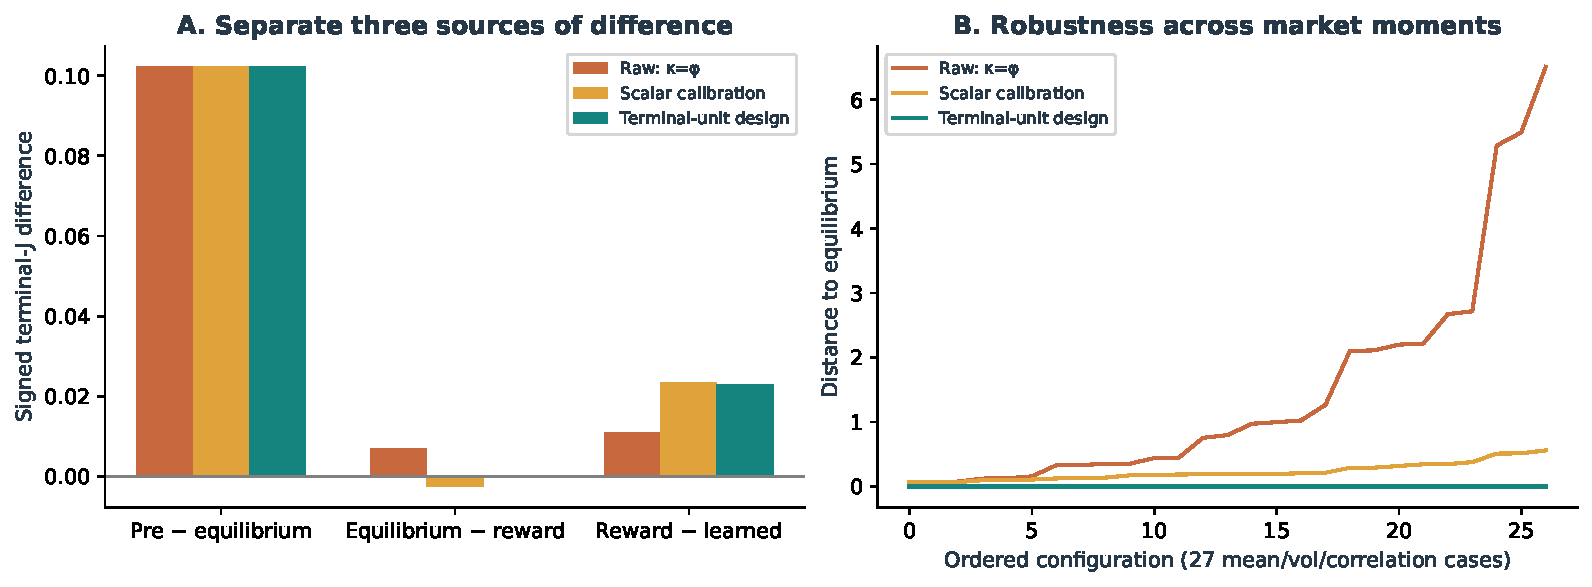
\includegraphics[width=\linewidth]{figures/09_decomposition_markets.pdf}
\caption{PRELIMINARY learning decomposition (left), NUMERICALLY VERIFIED moment sweep (right). Signed components must not be presented as three nonnegative losses. Ordered market curves compare each method's distribution of distances, not paired x-axis cases.}
\label{fig:09_decomposition_markets}
\end{figure}
Main limitations: analytically simple markets and unconstrained dollar positions; moment and model knowledge; oracle continuation in the dependent redesign; small exact constrained trees; five training seeds; no transaction-cost or historical replication. These are deliberate boundaries of the evidence.

The research contribution is therefore an exact, reproducible diagnostic and a conditional design result. It is stronger than an abstract framework, but narrower than a claim that a new reward generally improves financial RL.


\clearpage

\begin{thebibliography}{99}
\bibitem{ref1} Petter N. Kolm; Gordon Ritter. Dynamic Replication and Hedging: A Reinforcement Learning Approach. The Journal of Financial Data Science 1(1), 159--171 (2019). \url{https://doi.org/10.3905/jfds.2019.1.1.159}
\par\smallskip\noindent\emph{Source verification.} 16-page author manuscript at smallake.kr; figures are missing in this manuscript. Text and equations read; journal PDF unavailable. ``Automatic hedging in theory'', manuscript pp. 7--8, Eqs. (8)--(10), footnote 4; ``Automatic hedging in practice'', pp. 9--14, Exhibits 1--5.

\bibitem{ref2} Zhengyao Jiang; Dixing Xu; Jinjun Liang. A Deep Reinforcement Learning Framework for the Financial Portfolio Management Problem. arXiv preprint 1706.10059 (2017). \url{https://arxiv.org/abs/1706.10059}
\par\smallskip\noindent\emph{Source verification.} arXiv v2, 16 July 2017; saved PDF. \S{}\S{}2.2--2.4, \S{}4.2 Eqs. (21)--(22), \S{}4.3; Tables 1--2; \S{}6.

\bibitem{ref3} Hongyang Yang; Xiao-Yang Liu; Shan Zhong; Anwar Walid. Deep Reinforcement Learning for Automated Stock Trading: An Ensemble Strategy. Proceedings of the First ACM International Conference on AI in Finance (ICAIF), 8 pages (2020). \url{https://doi.org/10.1145/3383455.3422540}
\par\smallskip\noindent\emph{Source verification.} Columbia-hosted author manuscript; saved PDF. Do not use the later 2025 arXiv upload as a 2020 identifier. \S{}3.3 Eq. (4); \S{}5 ensemble selection; \S{}6.1 and Fig. 4; \S{}6.2.4 and Table 2.

\bibitem{ref4} John Moody; Matthew Saffell. Learning to Trade via Direct Reinforcement. IEEE Transactions on Neural Networks 12(4), 875--889 (2001). \url{https://doi.org/10.1109/72.935097}
\par\smallskip\noindent\emph{Source verification.} IDSIA-hosted 17-page manuscript, visually read because text encoding is corrupted. \S{}II-D, Eqs. (12)--(17), PDF pp. 3--4; \S{}III-A Eq. (31); \S{}IV-A, Fig. 5; \S{}IV-C.2, Fig. 8.

\bibitem{ref5} Lorenzo Bisi; Luca Sabbioni; Edoardo Vittori; Matteo Papini; Marcello Restelli. Risk-Averse Trust Region Optimization for Reward-Volatility Reduction. Proceedings of IJCAI-20, 4583--4589 (2020). \url{https://doi.org/10.24963/ijcai.2020/632}
\par\smallskip\noindent\emph{Source verification.} Published proceedings PDF, saved and read. \S{}3 Eqs. (3)--(6); \S{}\S{}4--5, Algorithm 1; \S{}7.1--7.2, Fig. 1(a)--(d).

\bibitem{ref6} Shangtong Zhang; Bo Liu; Shimon Whiteson. Mean-Variance Policy Iteration for Risk-Averse Reinforcement Learning. Proceedings of AAAI 35(12), 10905--10913 (2021). \url{https://doi.org/10.1609/aaai.v35i12.17302}
\par\smallskip\noindent\emph{Source verification.} arXiv:2004.10888v6, 7 April 2022; differs in date from published 2021 proceedings. ``Mean-Variance RL'', Eq. (2); ``Mean-Variance Policy Iteration'', Eqs. (3)--(4), Algorithm 1, Propositions 1--2; ``Experiments'', Table 1.

\bibitem{ref7} Haoran Wang; Xun Yu Zhou. Continuous-Time Mean-Variance Portfolio Selection: A Reinforcement Learning Framework. Mathematical Finance 30(4), 1273--1308 (2020). \url{https://doi.org/10.1111/mafi.12281}
\par\smallskip\noindent\emph{Source verification.} arXiv:1904.11392, saved 39-page preprint; section references refer to this version. \S{}2 Eq. (11); \S{}3 Theorems 1 and 3; \S{}4; \S{}5.1 Table 1, \S{}\S{}5.2--5.3.

\bibitem{ref8} Min Dai; Yuchao Dong; Yanwei Jia. Learning Equilibrium Mean-Variance Strategy. Mathematical Finance 33(4), 1166--1212 (2023). \url{https://doi.org/10.1111/mafi.12402}
\par\smallskip\noindent\emph{Source verification.} NUS RMI Working Paper 2021-02, March 2021, 52 pages, read via web PDF. Local download blocked; journal section numbering not asserted. Working version \S{}\S{}2--3, \S{}4.2 Theorem 2; \S{}5 Algorithm 1; \S{}6.1--6.2, Fig. 1.

\bibitem{ref9} Duan Li; Wan-Lung Ng. Optimal Dynamic Portfolio Selection: Multiperiod Mean-Variance Formulation. Mathematical Finance 10(3), 387--406 (2000). \url{https://doi.org/10.1111/1467-9965.00100}
\par\smallskip\noindent\emph{Source verification.} Journal PDF mirrored at tianjiablog.wordpress.com; saved. \S{}\S{}3--4, Theorems 1--2 (embedding); \S{}5 riskless-asset case.

\bibitem{ref10} Suleyman Basak; Georgy Chabakauri. Dynamic Mean-Variance Asset Allocation. The Review of Financial Studies 23(8), 2970--3016 (2010). \url{https://doi.org/10.1093/rfs/hhq028}
\par\smallskip\noindent\emph{Source verification.} Author thesis chapter 2, ``Dynamic Mean-Variance Asset Allocation'', read; journal full text unavailable. Chapter numbering is not journal numbering. Thesis chapter 2 \S{}2.2.2, Proposition 2.1, Eqs. (148)--(149); \S{}2.2.2 Remark 1; \S{}2.2.4; discrete-time extension in \S{}2.4.

\bibitem{ref11} Andrew Y. Ng; Daishi Harada; Stuart Russell. Policy Invariance under Reward Transformations: Theory and Application to Reward Shaping. Proceedings of ICML, 278--287 (1999). \url{https://ai.stanford.edu/~ang/papers/shaping-icml99.pdf}
\par\smallskip\noindent\emph{Source verification.} Author-hosted 10-page conference paper; visually read due to encoding. No DOI asserted. \S{}3 Theorem 1, Eq. (2), Corollary 2; \S{}4 Figures 1--2; Appendix A.

\bibitem{ref12} Tomas Björk; Agatha Murgoci. A Theory of Markovian Time-Inconsistent Stochastic Control in Discrete Time. Finance and Stochastics 18(3), 545--592 (2014). \url{https://doi.org/10.1007/s00780-014-0234-y}
\par\smallskip\noindent\emph{Source verification.} Publisher metadata and abstract only; full-text verification OPEN. Not counted as a paper fully read. Publisher abstract only; no theorem number or detailed comparison asserted.

\end{thebibliography}

\end{document}
